\documentclass[17pt, a2paper, portrait]{tikzposter}
\usepackage[utf8]{inputenc}

\title{Shawn A. Ross}
\author{Director, Data Science and eResearch}
%\date{\today}
\institute{Office of the DVCR, Macquarie University~\textbullet~{\tt shawn.ross@mq.edu.au\\
https://orcid.org/0000-0002-6492-9025} }

\usepackage{blindtext}
\usepackage{comment}
\usepackage{microtype}
\definecolor{mqRed}{HTML}{A6192E}
\definecolor{mqDeepRed}{HTML}{76232F}
\definecolor{mqBrightRed}{HTML}{D6001C}
\definecolor{mqMagenta}{HTML}{C6007E}
\definecolor{mqPurple}{HTML}{80225F}
\definecolor{mqCharcoal}{HTML}{373A36}
\definecolor{mqSand}{HTML}{D6D2C4}
\definecolor{mqBlack}{HTML}{000000}
\definecolor{mqWhite}{HTML}{FFFFFF}


\usetheme{Simple}
\usecolorpalette{Default}
\usecolorstyle[colorOne=mqCharcoal, colorTwo=mqRed, colorThree=mqDeepRed]{Denmark}

\titlegraphic{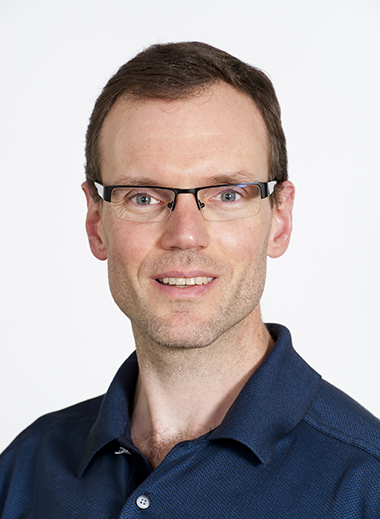
\includegraphics[width=0.1\linewidth]{images/Shawn_Ross.png}}

\makeatletter
\renewcommand\TP@maketitle{%
   \centering
    \tikz[remember picture,overlay]\node[scale=0.8,anchor=east,xshift=0.46\linewidth,yshift=2.85cm,inner sep=0pt] {%
       \@titlegraphic
    };
   \begin{minipage}[b]{0.8\linewidth}
        \centering
        \color{titlefgcolor}
        {\bfseries \Huge \sc \@title \par}
        \vspace*{1em}
        {\Large \@author \par}
        \vspace*{1em}
        { \@institute}
    \end{minipage}%
     \tikz[remember picture,overlay]\node[scale=0.8,anchor=east,xshift=0.18\linewidth,yshift=2.85cm,inner sep=0pt] {%
       \includegraphics[width=0.2\linewidth]{images/MQ_MAS_VER_RGB_REV.png}
    };
    
     
}
\makeatother

\begin{document}

\maketitle

\begin{columns}
\column{0.7}%
\block{My Research}{
\begin{itemize}
\item Landscape archaeology; 
\item Long-term history and archaeology of Greece and the Balkans; 
\item Small data / small science digital infrastructure; 
\item Infrastructure for field data capture across domains;
\item Socio-technical barriers to the adoption of new research technologies
\end{itemize}

}

\block{My digital toolbox}
{
\begin{itemize}
    \item OS: \textbf{Ubuntu} 
    \item Languages: \textbf{bash, R, Python (new to the latter but switching at the moment!}
    \item Code Development: \textbf{RStudio, Jupyter Notebooks}
    \item Reference Management: \textbf{Paperpile / Zotero -> Bib\TeX{}}
    \item Typesetting and Presentations: \textbf{OverLeaf and \LaTeX{}}
    \item GIS: \textbf{QGIS}
    \item Data cleaning: OpenRefine
    \item Photograph: Adobe suite (the only proprietary software I can't live without!)
    \item Vector graphics: Inkscape
\end{itemize}
}
\block{My favourite tools}
{
\textbf{Spatialite} for \textbf{SQLite}; \textbf{Git}; \textbf{*\TeX} (and overleaf) for typesetting \textit{everything}; \textbf{Floobits} for shared code composition; A nice mechanical keyboard for extra-clacky-typing; \textbf{SpiderOak ONE} for backups; \textbf{Bay Coffee} for a really consistent roast; \textbf{Tenjin} for Openstack based compute; \textbf{Yubikeys} for hardware security tokens; \textbf{Lastpass} for a password manager along with 5d6 and \textbf{Diceware} for generating passwords.  
}
\block{I've got my eye on}
{
 Pawsey's Nimbus deployment; Have I Been Pwned; the Australian Privacy Act; the New National Statement on Ethical Conduct in Human Research; Cloudstor and SWAN; AARnet's secure storage plans.

}
\column{0.3}%
\block{Logos}
{
\centering
\includegraphics[width=.95\linewidth]{images/logoWallResbaz2019.png}
}

% \block{~}
% {
%     \blindtext
% }

% 
%     \column{0.4}
%     \block{More text}{Text and more text}
    
%     \column{0.6}
%     \block{Something else}{Here, \blindtext \vspace{4cm}}
%     \note[
%         targetoffsetx=-9cm, 
%         targetoffsety=-6.5cm, 
%         width=0.5\linewidth
%         ]
%         {e-mail \texttt{sharelatex@sharelatex.com}}
% \end{columns}

% \begin{columns}
%     \column{0.5}
%     \block{A figure}
%     {
%         \begin{tikzfigure}
%             \includegraphics[width=0.4\textwidth]{images/lion-logo.png}
%         \end{tikzfigure}
%     }
%     \column{0.5}
%     \block{Description of the figure}{\blindtext}
\end{columns}


\node [above right,
       outer sep=0pt,
       minimum width=\paperwidth-2*\pgflinewidth,
       minimum height=0.5cm,
       align=center,font=\small] at ([shift={(0.5*\pgflinewidth,0.5*\pgflinewidth)}]bottomleft) {\tt{https://github.com/Denubis/Resbaz-2019-Poster} \includegraphics[height=14pt]{images/Cc-by-icon.png}\\
};


\end{document}
